\todo{services.tex}
\section{Services and Tools for Big Data}

\subsection{Traditional High Performance Computing}

The traditional high performance computing environment provied by queuing systems and Message Passing Interface (MPI) programs provide a suitable infrastructure not only for simulations, but also for the analysis of large data. However, considerable amount of work has to be put in place to optimize the available infarstructure for the problem doamin. This has been successfully demonstrated for many biological applications. Additinally the existance of a queuing system can provide some advantages when the available resources are utilized to a full extend and resource starvation exists while sharing the resources with other users. This has been esppecially useful to also support educational activities for clases with many users that for example want to test map reduce activities controled by a queing system as described in Section \ref{S:hadoop}.

\subsection{Virtual Large-Memory System}

One of the demands often posed in big data analysis it to place the data as much as possible into memory to speed up calculations and in some cases to fit the entire dataset into memore. However, this analysis may come at a cost as for example the use of HPC computing via MPI adds additional programming complexity within a cluster. Therefore it is desirable to virtualize the memory from multiple servers in a cluster to provide one big memory system that can be easily accessed by the underlying software. 
One such implementation, vSMP by ScaleMP \cite{www-scalemp}.
Experiments conducted on futureGrid using HPCC
benchmarks show only a 4-6\% drop in efficiency when compared to native
cluster performance \cite{las12fg-bookchapter}. This makes it feasable for many applications. ScaleMP is installed on the FutureGrid echo cluster that has 16 servers and can access up to 3TB in shared virtual memory.

\subsection{Infrastructure as a Service}



According to the manual FutureGrid provides a number of different
services. These services include:

\begin{enumerate}
\item OpenStack which includes a collection of open source components to deliver public and private clouds. These components currently include OpenStack Compute) OpenStack Object Storage, and OpenStack Image Service. OpenStack has received considerable momentum due to its openness and the support of companies. 

\item Nimbus which is an opensource service package that allows users to run virtual machines on FutureGrid hardware. Just as in Openstack users can upload their own virtual machine images or customize existing once. Nimbusnext to Eucalyptus is one of the earlier frameworks that make managing virtual machines easier.

\item Eucalyptus is an opensource software platform that implements IaaS-style cloud computing. Eucalyptus provides an Amazon Web Services (AWS) compliant EC2-based web service interface for interacting with the Cloud service.  Eucalyptus has been previously the dominant alternative to AWS  in academia. However, based on usage patterns in FutureGrid we believe it is replaced by OpenStack.

\item High Performance Computing can be defined as the application of supercomputing techniques to solve computational problems that are too large for standard computers or would take too much time. This is one of the more important features that the scientific community needs to achieve their projects. Naturally using HPC resouces and services is also useful in the area of Big Data. Sometimes big data needs big machines. Thus, using HPC may be an ovious choice.

\item Map Reduce …. TBD …

\end{enumerate}

Storage on FutureGrid has moderate size storage capability that will satisfy the users demand to compare and test someof the previously outlined services.

Information Services gather the information of the different elements that make up FutureGrid to provide accurate and complete knowledge of the computational environment. This information is presented using different web portals.

\begin{figure}[p]
  \centering
    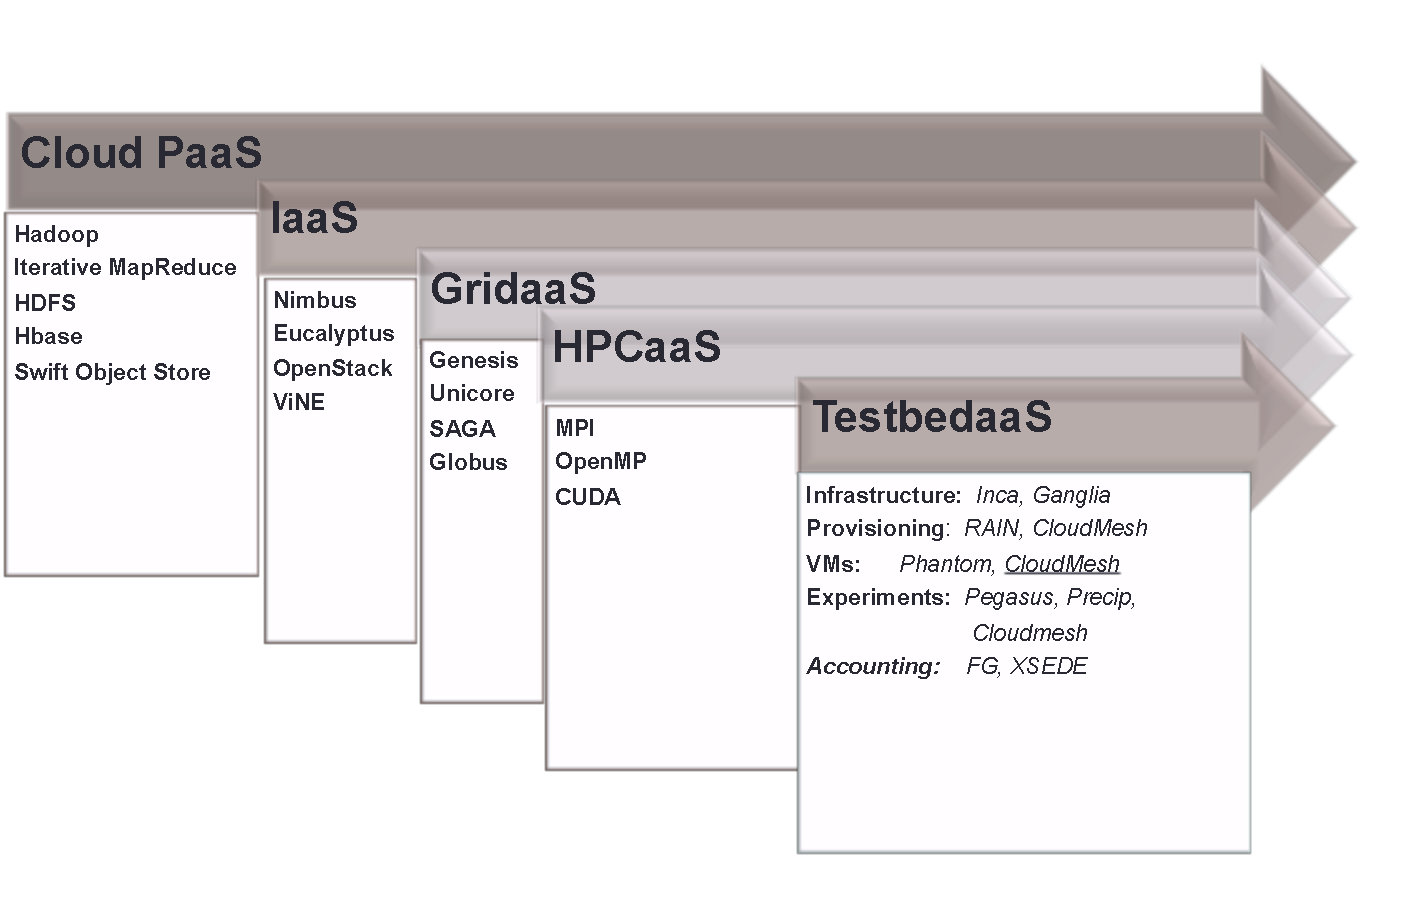
\includegraphics[width=0.9\textwidth]{images/user-services.pdf}
  \caption{FutureGrid High Level User Services.}
  ~\\
  \centering
  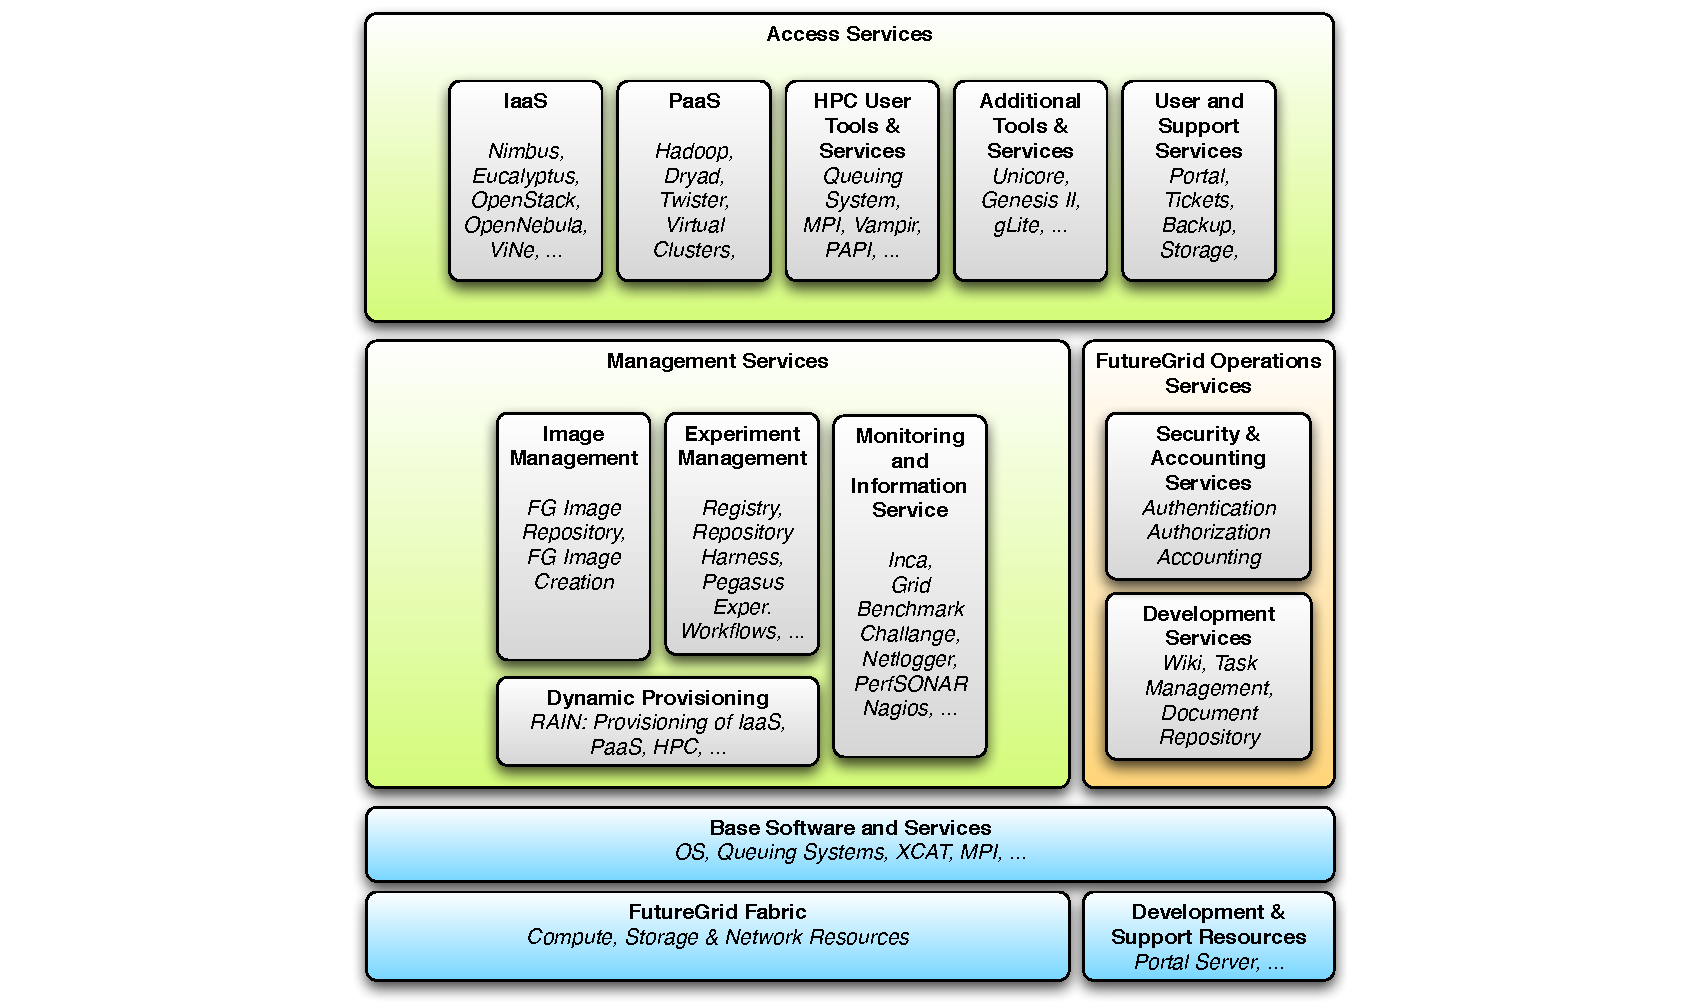
\includegraphics[width=0.9\textwidth]{images/architecture.pdf}
  \caption{Architecture.}
\end{figure}

\section{Hadoop}

\todo{reorganize hadoop section}
 
''The Apache Hadoop project develops opensource software for reliable, scalable, distributed computing.

The Apache Hadoop software library is a framework that allows for the distributed processing of large data sets across clusters of computers using simple programming models. It is designed to scale up from single servers to thousands of machines, each offering local computation and storage. Rather than rely on hardware to deliver highavailability, the library itself is designed to detect and handle failures at the application layer, so delivering a highlyavailable service on top of a cluster of computers, each of which may be prone to failures.
'' \cite{www/hadoop}

from sriram \cite{report/myhadoop}

\section{Hadoop}

Traditional HPC environments typically support batch job submissions
using resource management systems such as the TORQUE Resource Manager (also known as the
Portable Batch System – PBS) or the Sun Grid Engine (SGE). On the other hand, Hadoop
provides it own scheduling, and manages its own job and task submissions, and tracking.
Since both systems are designed to have complete control over the resources that they
manage, the challenge is how to enable users to run Hadoop jobs in a typical HPC
environment using a scheduler such as PBS or SGE. In this release, we support Hadoop
job submissions via PBS and SGE. However, this approach is equally feasible for other
schedulers such as Condor, as well.
Our approach is to configure Hadoop clusters “on-demand” by first requesting resources
for an Nnode Hadoop cluster via PBS. Once the resources are received, the Hadoop
configurations and environments are set up based on the set of resources provided by
PBS. The Hadoop Distributed File System (HDFS) can be configured in one of two ways
– in 1) transient (nonpersistent) or 2) persistent modes. In the nonpersistent mode, the
HDFS is set up to use local storage. In the persistent mode, the HDFS is set to
symbolically link to an external location that will be persistent – i.e. data from Hadoop
runs will continue to persist even after the Hadoop runs are complete. More details are as
follows.

\subsection{Details}

The prerequisite for myHadoop is a valid Hadoop installation – we recommend that you
use Hadoop version 0.20.2 since that is the only version of Hadoop that this package has
been tested with. Henceforth, we will refer to the location of the Hadoop installation as
HADOOP\_HOME. We will refer to the location of the myHadoop installation (i.e. this
package) as MY\_HADOOP\_HOME. The \$MY\_HADOOP\_HOME/pbs-example.sh shows
an example of how to use myHadoop with PBS. A similar script for SGE can be found in
\$MY\_HADOOP\_HOME/sge-example.sh.
A step-by-step process for using myHadoop is as follows.

\subsection{Initial Configuration}

Ensure that the environment variables inside \$MY\_HADOOP\_HOME/bin/setenv.sh are
set correctly. You can set your HADOOP\_HOME, and the locations for your HDFS data
and log directories using this script. You will need to update this script before you can
proceed further.
All the tuning parameters for Hadoop can be found in the \$MY\_HADOOP\_HOME/etc
directory. There is no need to edit any of the parameters, especially if you are not an
expert Hadoop user. If you are familiar with the various Hadoop parameters, you may
edit the parameters that fall outside the “DO NOT EDIT” sections.

\subsection{Request N nodes from the Scheduler}

Once the environment variables have been set correctly, we are ready to use myHadoop
using a regular PBS or SGE submission script. Your PBS script should contain the
following lines to initialize PBS as follows:

\begin{verbatim}
#!/bin/bash
#PBS -q <queue_name>
#PBS -N <job_name>
#PBS -l nodes=4:ppn=1
#PBS -o <output file>
#PBS -e <error_file>
#PBS -A <allocation>
#PBS -V
#PBS -M <user email>
#PBS -m abe
\end{verbatim}

In the above case, we are requesting 4 nodes. Note that you must set the processors per
node (ppn) to 1.
Your SGE script should contain the following lines to initialize SGE:

\begin{verbatim}
#!/bin/bash
#$ -V -cwd
#$ -N <job_name>
#$ -pe <queue_name> 4
#$ -o <output file>
#$ -e <error file>
#$ -S /bin/bash
\end{verbatim}

For SGE, there is one important rule to remember. The queue name specified above
should be preconfigured with an allocation\_rule set to 1 (one). This ensures that the
Hadoop cluster is set up such that multiple instances of the Hadoop daemons are not
scheduled on the same node.

\subsection{Set the myHadoop Environment}

Run the \$MY\_HADOOP\_HOME/bin/setenv.sh script (that you modified in Section 2.1)
to set all the environment variables required by myHadoop.
. \$MY\_HADOOP\_HOME/bin/setenv.sh
Set the HADOOP\_CONF\_DIR to the directory where Hadoop configs should be
generated – all configuration files for the Hadoop run will be picked up from here. Ensure
that this directory is accessible to all nodes – and a way to do this is to make sure that this
directory is on a shared file system such as NFS or Lustre.
export HADOOP\_CONF\_DIR=<configuration directory>

\subsection{Configure the myHadoop Cluster}

You can initialize and configure the Hadoop cluster by using the
\$MY\_HADOOP\_HOME/bin/pbs-configure.sh (or sge-configure.sh) script. You may
create a transient or persistent myHadoop cluster by changing the commandline
arguments as follows.
For a transient myHadoop cluster, configure it as follows (replace 4 with the total number
of nodes requested):
\$MY\_HADOOP\_HOME/bin/pbs-configure.sh -n 4 -c \$HADOOP\_CONF\_DIR
In this mode, you will have to copy all of your data into the myHadoop cluster after it is
configured, and copy out the results after the job is complete. All data will be
inaccessible from HDFS once the PBS job is complete.
Alternatively, you may set up a persistent myHadoop cluster by using the –p option, and
setting the BASE\_DIR for HDFS as follows:
\$MY\_HADOOP\_HOME/bin/pbs-configure.sh -n 4 -c \$HADOOP\_CONF\_DIR -p -d
<HDFS BASE\_DIR>
The BASE\_DIR should be on a directory accessible to all nodes, to ensure that the data
will not be cleaned up after job completion. For instance, the BASE\_DIR could be on a
Lustre file system. Note that, if N-node cluster is being created, then the BASE\_DIR
should have directories named 1, 2, … , N. The configuration script sets up symbolic
links from node I to the BASE\_DIR/I directory. When this mode is used, there is no need
to copy data back and forth from HDFS to another file system between runs.

\subsection{Format HDFS (if need be)}

If myHadoop is being used in transient mode, or if it is being used for the first time in
persistent mode, then you will have to format the HDFS as follows:
\$HADOOP\_HOME/bin/hadoop --config \$HADOOP\_CONF\_DIR namenode –format

\subsection{Run Hadoop Jobs}

You are now all set to start all the Hadoop daemons as follows:
\$HADOOP\_HOME/bin/start-all.sh
Once the daemons are all started up, you can start using Hadoop as usual. You may also
stage data in and out from HDFS, as required.

\subsection{Clean up}

Although, PBS or SGE may be set up to automatically clean up after your Hadoop job is
complete, it is always a good idea to stop all the Hadoop daemons, and use the cleanup
script to clean up after yourself.
\$HADOOP\_HOME/bin/stop-all.sh
\$MY\_HADOOP\_HOME/bin/pbs-cleanup.sh -n 4 OR
\$MY\_HADOOP\_HOME/bin/sge-cleanup.sh -n 4


\subsection{Hadoop}

My Hadoop

We have various platforms that support Hadoop on FutureGrid. MyHadoop is probably the easiest solution offered for you. It provides the advantage that it is integrated into the queuing system and allows hadoop jobs to be run as batch job. This is of especial interest for classes that may run quickly out of resources if every students wants to run their hadoop application at the same time.



MapReduce is a programming model developed by Google. Their definition of MapReduce is as follows: “MapReduce is a programming model and an associated implementation for processing and generating large data sets. Users specify a map function that processes a key/value pair to generate a set of intermediate key/value pairs, and a reduce function that merges all intermediate values associated with the same intermediate key.” For more information about MapReduce, please see the Google paper here.

The Apache Hadoop Project provides an open source implementation of MapReduce and HDFS (Hadoop Distributed File System).

This tutorial illustrates how to run Apache Hadoop thru the batch systems on FutureGrid using the MyHadoop tool.

\subsubsection{myHadoop on FutureGrid}

MyHadoop is a set of scripts that configure and instantiate Hadoop as a batch job.

myHadoop 0.20.2 is currently installed on Alamo, Hotel, India, and Sierra FutureGrid systems.

